\section{Nonparametric estimation of distributions and densities}\label{sec:A-kde}

The estimators of the previous sections are parametric, in the sense that a finite-dimensional $\theta$ indexes
the model. Several of the book's estimators instead recover an unknown distribution without a parametric family. The
structural auction literature is the main user. The value distribution of an ascending auction is
recovered from the distribution of transaction prices. In a first-price auction it is recovered from the
distribution and density of bids (\cref{ch:auction-empirics}). Bidding
rings and procurement auctions with unobserved heterogeneity add a deconvolution step
(\cref{ch:collusion-evidence}), and hedonic demand models use nonparametric regression
(\cref{ch:discrete}). This section develops the estimators of distribution functions and densities on
which these applications rest. \Cref{sec:A-npreg} turns to regression, deconvolution and bounds.

The notation is local to these two sections. A \emph{kernel} $\mathcal{K}$ is a weighting function,
$h>0$ is a \emph{bandwidth}, and $\mathcal{K}_h(u)=\frac{1}{h}\mathcal{K}(\frac{u}{h})$. The constants
$\mu_2=\int u^2\mathcal{K}(u)\,\dd u$ and $\kappa_2=\int\mathcal{K}(u)^2\,\dd u$ are the second moment
and the roughness of the kernel, and $R$ counts the derivatives of the target function. In the auction
applications we follow \citet{GuerrePerrigneVuong2000}, hereafter GPV, and write $L$ for the number of
auctions. In these two sections $L$ is therefore neither a Lerner index nor a number of instruments. Each auction has $N$
bidders (GPV write $I$), bids are $B_{il}$, and the bid distribution and density are $G$ and $g$.

\subsection{The empirical distribution function}\label{sec:A-ecdf}

Let $X_1,\dots,X_n$ be independent draws from a distribution function $F$ on $\R$. The
\emph{empirical distribution function} puts mass $\frac{1}{n}$ on each observation:
\begin{equation}\label{eq:A-ecdf}
\hat F_n(x)=\frac{1}{n}\sum_{i=1}^{n}\indic\{X_i\le x\}.
\end{equation}

\begin{proposition}[Properties of the empirical distribution function]\label{prop:A-ecdf}
Let $X_1,\dots,X_n$ be i.i.d.\ with distribution function $F$.
\begin{enumerate}[label=(\roman*)]
\item For every $x$, $\E[\hat F_n(x)]=F(x)$ and $\Var(\hat F_n(x))=\frac{F(x)(1-F(x))}{n}$.
\item For every $x$, $\sqrt n(\hat F_n(x)-F(x))\xrightarrow{d}N(0,F(x)(1-F(x)))$.
\item (Glivenko-Cantelli) $\sup_x|\hat F_n(x)-F(x)|\to0$ almost surely.
\item (Dvoretzky-Kiefer-Wolfowitz) For every $\epsilon>0$,
$\Pr\left(\sup_x|\hat F_n(x)-F(x)|>\epsilon\right)\le2e^{-2n\epsilon^2}$.
\end{enumerate}
\end{proposition}

\begin{proof}
For fixed $x$ the indicators $\indic\{X_i\le x\}$ are i.i.d.\ Bernoulli variables with success probability
$F(x)$. Their mean is $F(x)$ and their variance is $F(x)(1-F(x))$. Averaging $n$ of them divides the
variance by $n$, which proves (i). Part (ii) is the Lindeberg-L\'evy central limit theorem applied to the
same Bernoulli average. Parts (iii) and (iv) are classical uniform results. The constant 2 in front of
the exponential in (iv) is due to \citet{Massart1990}.
\end{proof}

Part (iv) yields a confidence band that holds for all $x$ at once. Setting $2e^{-2n\epsilon^2}=\alpha$
gives $\epsilon_\alpha=\sqrt{\frac{\ln(\frac{2}{\alpha})}{2n}}$, and the band
$\hat F_n(x)\pm\epsilon_\alpha$ contains the whole function $F$ with probability at least $1-\alpha$. With
$n=200$ and $\alpha=0.05$ the half-width is about 0.096. The band needs no smoothing and no
estimate of a density, which makes the empirical distribution function the natural first step of every
estimator in this section.

\casehead{Order-statistic inversion}
In a second-price or ascending auction with symmetric independent private values, the price equals
the second-highest value (\cref{ch:auction-theory}). Suppose we observe only prices $w_l$ from $L_N$
auctions with $N$ bidders each. The price is $v_{(N-1:N)}$, and its distribution function is
\begin{equation}\label{eq:A-phiN}
F_w(v)=\Pr\left(v_{(N-1:N)}\le v\right)=\phi_N(F(v)),\qquad \phi_N(x)=Nx^{N-1}(1-x)+x^N .
\end{equation}
The second-highest value lies below $v$ exactly when at least $N-1$ of the $N$ values do. The first term
of $\phi_N$ is the probability that exactly $N-1$ values lie below $v$, and the second that all $N$ do.
The derivative is
\begin{equation*}
\phi_N'(x)=N(N-1)x^{N-2}(1-x)-Nx^{N-1}+Nx^{N-1}=N(N-1)x^{N-2}(1-x),
\end{equation*}
which is positive on $(0,1)$. So $\phi_N$ is a strictly increasing bijection of $[0,1]$, and
$F(v)=\phi_N^{-1}(F_w(v))$. More generally, the $k$-th lowest of $N$ i.i.d.\ draws has distribution
function
\begin{equation}\label{eq:A-orderstat}
F_{(k:N)}(v)=\frac{N!}{(N-k)!\,(k-1)!}\int_0^{F(v)}t^{k-1}(1-t)^{N-k}\,\dd t ,
\end{equation}
which is strictly increasing in $F(v)$ \citep[eq.~(5)]{AtheyHaile2002}. Any single order statistic with
known $N$ therefore identifies $F$, and \eqref{eq:A-phiN} is the case $k=N-1$.

The plug-in estimator replaces $F_w$ by the empirical distribution function of the prices,
$\hat F(v)=\phi_N^{-1}(\hat F_w(v))$, computed by bisection at each $v$.

\begin{proposition}[Order-statistic inversion]\label{prop:A-os-inversion}
Let $w_1,\dots,w_{L_N}$ be i.i.d.\ prices from $N$-bidder auctions and let $0<F(v)<1$. Then
$\hat F(v)\xrightarrow{p}F(v)$ and
\begin{equation}\label{eq:A-os-avar}
\sqrt{L_N}\left(\hat F(v)-F(v)\right)\xrightarrow{d}
N\!\left(0,\ \frac{F_w(v)(1-F_w(v))}{\phi_N'(F(v))^2}\right).
\end{equation}
\end{proposition}

\begin{proof}
Consistency follows from \cref{prop:A-ecdf}(i) and the continuity of $\phi_N^{-1}$. The inverse
function theorem gives $\frac{\dd}{\dd y}\phi_N^{-1}(y)=\frac{1}{\phi_N'(\phi_N^{-1}(y))}$, which is
finite because $\phi_N'(F(v))>0$. The delta method (\cref{thm:A-delta}) applied to
\cref{prop:A-ecdf}(ii) multiplies the asymptotic variance $F_w(1-F_w)$ by the square of this
derivative.
\end{proof}

The variance in \eqref{eq:A-os-avar} measures what is lost by observing one order statistic. If all $N$
values of each auction were recorded, the empirical distribution function of the $NL_N$ values would
have asymptotic variance $\frac{F(1-F)}{N}$ per auction. With $N=4$ and $F(v)=0.5$, the price-only
variance is 0.0955 against 0.0625, a ratio of 1.53. At $F(v)=0.2$ the ratio is 4.49, and with $N=6$ at
the same point it reaches 40.6. The price is the second-highest value, so it carries little information about the lower
tail, and the loss grows with $N$. These numbers come from \texttt{kernel\_constants.py}.

Two extensions matter in practice. First, the inversion delivers one estimate of $F$ for each $N$ in the
data. If participation varies independently of values, all these estimates must coincide, which is a
testable restriction \citep[Theorem~1]{AtheyHaile2002}. The estimates from different $N$ are
independent, so a Wald-type comparison at a point $v$ divides their difference by the square root of the
sum of the two variances in \eqref{eq:A-os-avar}. Second, with a binding reserve price $r$ the price is
$\max\{v_{(N-1:N)},r\}$, and $F$ is identified only above $r$. \Cref{ch:auction-empirics} develops the
identification argument, and \cref{sec:A-partialid} returns to ascending auctions in which recorded bids
are not values.

\subsection{The kernel density estimator}\label{sec:A-kde-estimator}

A histogram estimates a density by counting observations in bins of width $2h$. It depends on the bin
origin, and it is discontinuous. The kernel estimator centers a smooth bump on each observation
instead \citep{Rosenblatt1956,Parzen1962}:
\begin{equation}\label{eq:A-kde}
\hat f_h(x)=\frac{1}{nh}\sum_{i=1}^{n}\mathcal{K}\!\left(\frac{x-X_i}{h}\right)
=\frac{1}{n}\sum_{i=1}^{n}\mathcal{K}_h(x-X_i).
\end{equation}
With the uniform kernel $\mathcal{K}(u)=\frac{1}{2}\indic\{|u|\le1\}$, $\hat f_h(x)$ is the share of
observations within $h$ of $x$ divided by $2h$, a histogram whose bin moves with $x$.

\begin{definition}[Second-order kernel]\label{def:A-kernel}
A \emph{second-order kernel} is a bounded function $\mathcal{K}$ with $\int\mathcal{K}(u)\,\dd u=1$,
$\int u\mathcal{K}(u)\,\dd u=0$, $0<\mu_2=\int u^2\mathcal{K}(u)\,\dd u<\infty$ and
$\kappa_2=\int\mathcal{K}(u)^2\,\dd u<\infty$. A bounded symmetric density with finite variance is a
second-order kernel.
\end{definition}

\begin{assumption}[Pointwise kernel asymptotics]\label{ass:A-kde}
The draws $X_1,\dots,X_n$ are i.i.d.\ with density $f$. In a neighborhood of the point $x$, $f$ is twice
continuously differentiable with bounded second derivative. The kernel is second order, and the bandwidth
satisfies $h\to0$ and $nh\to\infty$.
\end{assumption}

\begin{proposition}[Bias and variance of the kernel density estimator]\label{prop:A-kde-bias-var}
Under \cref{ass:A-kde},
\begin{equation}\label{eq:A-kde-bias-var}
\E[\hat f_h(x)]-f(x)=\frac{h^2}{2}\mu_2f''(x)+o(h^2),\qquad
\Var(\hat f_h(x))=\frac{f(x)\kappa_2}{nh}+o\!\left(\frac{1}{nh}\right).
\end{equation}
\end{proposition}

\begin{proof}
\emph{Bias.} The summands of \eqref{eq:A-kde} are i.i.d., so
\begin{equation*}
\E[\hat f_h(x)]=\int\frac{1}{h}\mathcal{K}\!\left(\frac{x-y}{h}\right)f(y)\,\dd y
=\int\mathcal{K}(u)f(x-hu)\,\dd u ,
\end{equation*}
where we substituted $y=x-hu$ and $\dd y=-h\,\dd u$. A second-order Taylor expansion with mean-value
point $\tilde x_u$ between $x$ and $x-hu$ gives
\begin{equation*}
f(x-hu)=f(x)-huf'(x)+\frac{h^2u^2}{2}f''(\tilde x_u).
\end{equation*}
Integrating against $\mathcal{K}$, the first term returns $f(x)$ and the second vanishes because
$\int u\mathcal{K}=0$. The third equals $\frac{h^2}{2}\int u^2\mathcal{K}(u)f''(\tilde x_u)\,\dd u$, which
is $\frac{h^2}{2}\mu_2f''(x)+o(h^2)$ by continuity of $f''$ and dominated convergence.

\emph{Variance.} Again by independence,
\begin{equation*}
\Var(\hat f_h(x))=\frac{1}{n}\left\{\E\left[\mathcal{K}_h(x-X)^2\right]-\left(\E[\mathcal{K}_h(x-X)]\right)^2\right\}.
\end{equation*}
The same substitution gives
$\E[\mathcal{K}_h(x-X)^2]=\frac{1}{h}\int\mathcal{K}(u)^2f(x-hu)\,\dd u=\frac{f(x)\kappa_2}{h}+O(1)$.
The squared mean is $f(x)^2+O(h^2)=O(1)$. Hence
$\Var(\hat f_h(x))=\frac{f(x)\kappa_2}{nh}+O(\frac{1}{n})$, and $\frac{1}{n}=o(\frac{1}{nh})$ because
$h\to0$.
\end{proof}

The proposition displays the basic trade-off of nonparametric estimation. A small bandwidth averages
few observations, so the variance is large. A large bandwidth averages over a region where $f$ curves,
so the bias is large. The variance is of order $\frac{1}{nh}$ because only about $2nhf(x)$ observations
fall in the kernel window, which is slower than the parametric $\frac{1}{n}$. Under the same conditions
a Lindeberg argument gives
$\sqrt{nh}\,(\hat f_h(x)-\E[\hat f_h(x)])\xrightarrow{d}N(0,f(x)\kappa_2)$.

\casehead{Optimal bandwidth}
The \emph{mean integrated squared error} is
$\mathrm{MISE}(h)=\E\int(\hat f_h(x)-f(x))^2\,\dd x$, the integral of squared bias plus variance.
Integrating the leading terms of \eqref{eq:A-kde-bias-var} and using $\int f=1$ gives the
\emph{asymptotic MISE}
\begin{equation}\label{eq:A-amise}
\mathrm{AMISE}(h)=\frac{h^4}{4}\mu_2^2\,\mathcal{R}(f'')+\frac{\kappa_2}{nh},\qquad
\mathcal{R}(f'')=\int f''(x)^2\,\dd x .
\end{equation}
The first-order condition $h^3\mu_2^2\mathcal{R}(f'')-\frac{\kappa_2}{nh^2}=0$ yields
\begin{equation}\label{eq:A-hstar}
h^*=\left[\frac{\kappa_2}{\mu_2^2\,\mathcal{R}(f'')\,n}\right]^{\frac{1}{5}} .
\end{equation}
At $h^*$ the squared-bias term equals one quarter of the variance term, so
\begin{equation*}
\mathrm{AMISE}(h^*)=\frac{5}{4}\,\frac{\kappa_2}{nh^*}
=\frac{5}{4}\left(\sqrt{\mu_2}\,\kappa_2\right)^{\frac{4}{5}}\mathcal{R}(f'')^{\frac{1}{5}}\,n^{-\frac{4}{5}} .
\end{equation*}
The optimal bandwidth shrinks like $n^{-\frac{1}{5}}$ and the error falls like $n^{-\frac{4}{5}}$, against
$n^{-1}$ for a correctly specified parametric model.

\casehead{Silverman's rule of thumb}
The unknown $\mathcal{R}(f'')$ in \eqref{eq:A-hstar} can be replaced by its value for a reference
density. Take $f$ normal with variance $\sigma^2$ and the Gaussian kernel, for which $\mu_2=1$ and
$\kappa_2=\frac{1}{2\sqrt\pi}$. Write $f(x)=\frac{1}{\sigma}\phi(\frac{x}{\sigma})$ with $\phi$ the
standard normal density. Then $f''(x)=\sigma^{-3}\phi''(\frac{x}{\sigma})$ and
$\phi''(u)=(u^2-1)\phi(u)$, so
\begin{equation*}
\mathcal{R}(f'')=\sigma^{-5}\int(u^2-1)^2\phi(u)^2\,\dd u .
\end{equation*}
Now $\phi(u)^2=\frac{1}{2\sqrt\pi}\,\psi(u)$, where $\psi$ is the $N(0,\frac{1}{2})$ density. For
$U\sim N(0,\frac{1}{2})$ we have $\E[U^2]=\frac{1}{2}$ and $\E[U^4]=\frac{3}{4}$, so
$\E[(U^2-1)^2]=\frac{3}{4}-1+1=\frac{3}{4}$. Therefore
\begin{equation*}
\mathcal{R}(f'')=\frac{3}{8\sqrt\pi\,\sigma^5},\qquad
(h^*)^5=\frac{\frac{1}{2\sqrt\pi}}{\frac{3}{8\sqrt\pi\,\sigma^5}\,n}=\frac{4}{3}\,\frac{\sigma^5}{n},
\end{equation*}
and
\begin{equation}\label{eq:A-silverman}
h_{\mathrm{ROT}}=\left(\frac{4}{3}\right)^{\frac{1}{5}}\sigma n^{-\frac{1}{5}}\approx1.06\,\sigma n^{-\frac{1}{5}} .
\end{equation}
This is the \emph{rule of thumb} of \citet{Silverman1986}, with $\sigma$ replaced by the sample standard
deviation. It is optimal for normal data and oversmooths densities with more curvature, such as
multimodal ones, because those have larger $\mathcal{R}(f'')$.

\casehead{Choice of kernel}
The kernel enters \eqref{eq:A-hstar} only through $\delta_{\mathcal{K}}=(\frac{\kappa_2}{\mu_2^2})^{\frac{1}{5}}$,
and the minimized AMISE only through $\sqrt{\mu_2}\,\kappa_2$. Two consequences follow. A bandwidth
rule derived for one kernel converts to another kernel by the factor
$\frac{\delta_{\mathcal{K}}}{\delta_{\phi}}$, whatever $f$ is. And kernels differ little in efficiency
once their bandwidths are scaled correctly. \Cref{tab:A-kernels} reports the constants. Among nonnegative
kernels the Epanechnikov kernel minimizes $\sqrt{\mu_2}\,\kappa_2$, and every other kernel in the table
attains at least 92.9 percent of its efficiency. The restriction to nonnegative kernels matters, because
\cref{def:A-kernel} allows negative values. Put weight $\lambda$ on the Epanechnikov kernel and $1 - \lambda$
on a bounded kernel of order four with compact support (\cref{sec:A-kde-higher}). The mixture is a second-order
kernel with $\mu_2 = \frac{\lambda}{5}$ and bounded $\kappa_2$, so its criterion tends to zero as $\lambda \to 0$.

\begin{table}[htbp]
\centering
\caption{Second-order kernels and their constants}\label{tab:A-kernels}
\begin{tabular}{lccccccc}
\toprule
Kernel & $\mathcal{K}(u)$ & $\mu_2$ & $\kappa_2$ & $\int\mathcal{K}'(u)^2\dd u$ & $\int_0^\infty u\mathcal{K}(u)\dd u$
 & $\frac{\delta_{\mathcal{K}}}{\delta_\phi}$ & Efficiency \\
\midrule
Uniform & $\frac{1}{2}$ & $\frac{1}{3}$ & $\frac{1}{2}$ & n.a. & $\frac{1}{4}$ & 1.740 & 0.930 \\[2pt]
Epanechnikov & $\frac{3}{4}(1-u^2)$ & $\frac{1}{5}$ & $\frac{3}{5}$ & $\frac{3}{2}$ & $\frac{3}{16}$ & 2.214 & 1.000 \\[2pt]
Biweight & $\frac{15}{16}(1-u^2)^2$ & $\frac{1}{7}$ & $\frac{5}{7}$ & $\frac{15}{7}$ & $\frac{5}{32}$ & 2.623 & 0.994 \\[2pt]
Triweight & $\frac{35}{32}(1-u^2)^3$ & $\frac{1}{9}$ & $\frac{350}{429}$ & $\frac{35}{11}$ & $\frac{35}{256}$ & 2.978 & 0.987 \\[2pt]
Gaussian & $\phi(u)$ & $1$ & $\frac{1}{2\sqrt\pi}$ & $\frac{1}{4\sqrt\pi}$ & $\frac{1}{\sqrt{2\pi}}$ & 1.000 & 0.951 \\
\bottomrule
\end{tabular}
\par\smallskip
\begin{minipage}{0.97\textwidth}
\footnotesize Notes: the first four kernels are zero outside $|u|\le1$. The column
$\frac{\delta_{\mathcal{K}}}{\delta_\phi}$ is the factor that converts a bandwidth rule for the Gaussian
kernel into the corresponding rule for kernel $\mathcal{K}$, with
$\delta_{\mathcal{K}}=(\frac{\kappa_2}{\mu_2^2})^{\frac{1}{5}}$. Efficiency is $\sqrt{\mu_2}\,\kappa_2$ of
the Epanechnikov kernel divided by $\sqrt{\mu_2}\,\kappa_2$ of the kernel in the row. It is the ratio of
sample sizes that gives the two kernels the same minimized AMISE. The
derivative roughness $\int\mathcal{K}'^2$ enters the variance of density-derivative estimators
(\cref{prop:A-kde-derivative}). The uniform kernel is not differentiable. All constants are computed
exactly with sympy in \texttt{kernel\_constants.py}.
\end{minipage}
\end{table}

The auction literature uses the triweight kernel almost exclusively. It has compact support, so
trimmed observations drop out of the estimate, and it is continuously differentiable on the whole line,
including the end points of its support. \citet[p.~532]{GuerrePerrigneVuong2000} chose it to satisfy
their kernel assumptions. \citet[p.~180]{LiPerrigneVuong2002} and \citet[Section~4.3]{Krasnokutskaya2011}\footnote{We use the
working-paper version of \citet{Krasnokutskaya2011} dated May 24, 2004 (PIER Working Paper 05-006), and equation,
section, lemma and proposition numbers refer to it.}
give the differentiability at the boundary as the reason. These authors also illustrate the conversion
factor. \citeauthor{LiPerrigneVuong2002} and \citeauthor{Krasnokutskaya2011} set the bandwidth constant
to $2.978\times1.06\,\hat\sigma$, and 2.978 is the triweight entry in the
$\frac{\delta_{\mathcal{K}}}{\delta_\phi}$ column. \citet[p.~532]{GuerrePerrigneVuong2000} and
\citet[p.~749]{Asker2010} use $1.06\,\hat\sigma$ with the same kernel, a bandwidth about one third of the
normal-reference rule for that kernel.

The exponents of the sample size also differ across these papers. GPV set $h_g=1.06\,\hat\sigma_b(NL)^{-\frac{1}{5}}$
for the bid density, with $\hat\sigma_b$ the standard deviation of the bids and $NL$ the number of bids (p.~532).
\citet[p.~749]{Asker2010} uses $1.06\,\hat\sigma n^{-\frac{1}{6}}$ for densities and $1.06\,\hat\sigma n^{-\frac{1}{5}}$
for kernel-smoothed distribution functions. \citet[Section~4.3]{Krasnokutskaya2011} uses
$2.978\times1.06\,\hat\sigma L^{-\frac{1}{6}}$, with $L$ her sample size and $\hat\sigma$ the standard deviation of
the log of one plus the bids, and says that she follows GPV. The rates of \cref{sec:A-kde-higher} explain the pattern. With $R$
derivatives of the value density and $d$ continuous covariates, GPV's bandwidths for the bid distribution and the bid
density shrink like $L^{-\frac{1}{2R+d+2}}$ and $L^{-\frac{1}{2R+d+3}}$, up to logarithms. With $R=1$ and no
covariates the density exponent is $-\frac{1}{5}$, GPV's own choice. With $R=1$ and $d=1$ the two exponents are
$-\frac{1}{5}$ and $-\frac{1}{6}$, the pair that Asker uses. Neither Asker nor Krasnokutskaya derives an exponent. In a
one-dimensional problem $L^{-\frac{1}{6}}$ shrinks more slowly than $L^{-\frac{1}{5}}$, so their bandwidths oversmooth
slightly relative to GPV's rule. Oversmoothing lowers the variance of $\hat g$ at the cost of more bias.

\Cref{fig:A-kde} illustrates the trade-off with a bimodal density,
$f=0.6\,N(0,1)+0.4\,N(2.5,0.5^2)$, and $n=200$. Panel (a) shows one sample. Halving the optimal
bandwidth produces spurious bumps, and doubling it blurs the two modes into a plateau. Panel (b) plots
the exact integrated squared bias, integrated variance and MISE against $h$, with Monte Carlo averages
over 1,000 samples as markers. The exact MISE is minimized at $h^*=0.291$, where the integrated
squared bias is 0.0014 and the integrated variance 0.0039. The AMISE formula \eqref{eq:A-hstar} gives
0.262. Its quartic bias term overstates the bias at large $h$, which pulls the AMISE minimizer to the
left.

\begin{figure}[htbp]
\centering
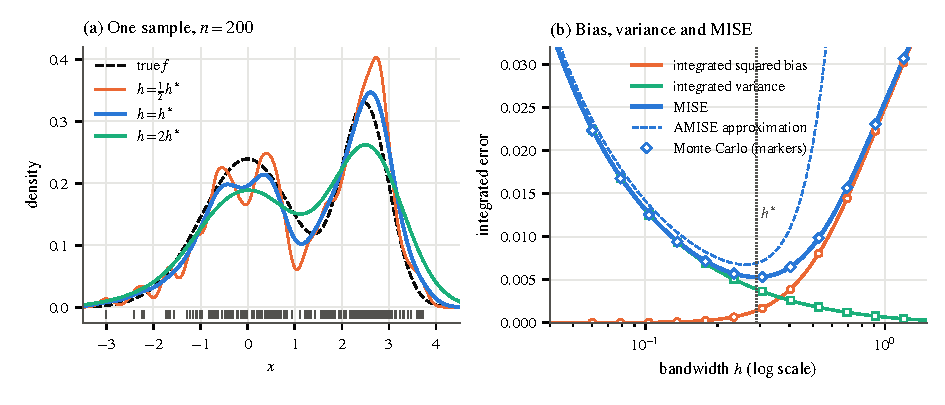
\includegraphics[width=\textwidth]{figures/appA/kde.pdf}
\caption{Bandwidth choice for a kernel density estimator. The true density is
$0.6\,N(0,1)+0.4\,N(2.5,0.5^2)$, the kernel is Gaussian and $n=200$. (a) One sample (the
median of 101 fresh samples by integrated squared error at $h^*$), with estimates at
$\frac{1}{2}h^*$, $h^*$ and $2h^*$, where $h^*=0.291$ minimizes the exact MISE. (b) Exact
integrated squared bias, integrated variance and MISE (solid lines), the AMISE approximation
\eqref{eq:A-amise} (dashed) and Monte Carlo averages over 1,000 samples (markers). Seed 20261022,
script \texttt{kde\_demo.py}.}
\label{fig:A-kde}
\end{figure}

\subsection{Smoothness, higher-order kernels and derivatives}\label{sec:A-kde-higher}

The $h^2$ bias of \cref{prop:A-kde-bias-var} comes from the second moment of the kernel. If $f$ has more
derivatives, kernels with more vanishing moments reduce the bias further.

\begin{definition}[Kernel of order $R$]\label{def:A-kernel-order}
A kernel $\mathcal{K}$ is of \emph{order} $R\ge2$ if $\int\mathcal{K}=1$,
$\mu_j=\int u^j\mathcal{K}(u)\,\dd u=0$ for $j=1,\dots,R-1$, and $0<|\mu_R|<\infty$.
\end{definition}

If $f$ has $R$ bounded continuous derivatives near $x$ and $\mathcal{K}$ is of order $R$, the expansion in
the proof of \cref{prop:A-kde-bias-var}, carried to order $R$, gives
\begin{equation}\label{eq:A-kde-bias-R}
\E[\hat f_h(x)]-f(x)=\sum_{j=1}^{R}\frac{(-h)^j}{j!}\mu_jf^{(j)}(x)+o(h^R)
=\frac{(-h)^R}{R!}\mu_Rf^{(R)}(x)+o(h^R).
\end{equation}
The variance is unchanged at order $\frac{1}{nh}$. Balancing $h^{2R}$ against $\frac{1}{nh}$ gives
$h\propto n^{-\frac{1}{2R+1}}$ and a root mean squared error of order $n^{-\frac{R}{2R+1}}$.
\citet{Stone1982} showed that $(\frac{n}{\log n})^{\frac{R}{2R+1}}$ is the best possible rate for
estimating such a density uniformly over a compact set. The logarithm is the price of uniformity.

For $R>2$ the kernel must take negative values, since $\mu_2=0$ is impossible for a nonnegative
function. Density estimates can then be negative. In the auction setting this has a concrete cost. A
negative estimated bid density produces pseudo-values below the corresponding bids, so
\citet[p.~180]{LiPerrigneVuong2002} keep second-order kernels in their three-bidder design even though
their theory calls for order three.

\casehead{Derivatives of a density}
Differentiating \eqref{eq:A-kde} gives an estimator of the derivative,
\begin{equation}\label{eq:A-kde-deriv}
\hat f_h'(x)=\frac{1}{nh^2}\sum_{i=1}^{n}\mathcal{K}'\!\left(\frac{x-X_i}{h}\right).
\end{equation}

\begin{proposition}[Rate for a density derivative]\label{prop:A-kde-derivative}
Let $\mathcal{K}$ be a continuously differentiable kernel of order $R$ that vanishes outside $[-1,1]$, and
let $f$ have $R+1$ bounded continuous derivatives near $x$. If $h\to0$ and $nh^3\to\infty$, then
\begin{equation*}
\E[\hat f_h'(x)]-f'(x)=\frac{(-h)^R}{R!}\mu_Rf^{(R+1)}(x)+o(h^R),\qquad
\Var(\hat f_h'(x))=\frac{f(x)\int\mathcal{K}'(u)^2\dd u}{nh^3}+o\!\left(\frac{1}{nh^3}\right).
\end{equation*}
The mean squared error is minimized by $h\propto n^{-\frac{1}{2R+3}}$, and the root mean squared error is
then of order $n^{-\frac{R}{2R+3}}$.
\end{proposition}

\begin{proof}
\emph{Bias.} Substituting $y=x-hu$,
\begin{equation*}
\E[\hat f_h'(x)]=\frac{1}{h}\int\mathcal{K}'(u)f(x-hu)\,\dd u .
\end{equation*}
Integration by parts, with $\mathcal{K}(\pm1)=0$ and $\frac{\dd}{\dd u}f(x-hu)=-hf'(x-hu)$, turns this into
$\int\mathcal{K}(u)f'(x-hu)\,\dd u$. This is the expectation of a kernel estimator of $f'$, and
\eqref{eq:A-kde-bias-R} applied to $f'$ gives the bias.

\emph{Variance.} Each summand of \eqref{eq:A-kde-deriv} is $\frac{1}{h^2}\mathcal{K}'(\frac{x-X_i}{h})$.
Its second moment is
\begin{equation*}
\frac{1}{h^4}\int\mathcal{K}'\!\left(\frac{x-y}{h}\right)^2f(y)\,\dd y=\frac{1}{h^3}\int\mathcal{K}'(u)^2f(x-hu)\,\dd u
=\frac{f(x)\int\mathcal{K}'^2}{h^3}+o\!\left(\frac{1}{h^3}\right),
\end{equation*}
while its squared mean is $O(1)$. Dividing by $n$ gives the variance.

\emph{Rate.} The mean squared error is $c_1h^{2R}+\frac{c_2}{nh^3}$ to first order. Its minimizer solves
$2Rc_1h^{2R-1}=\frac{3c_2}{nh^4}$, so $h\propto n^{-\frac{1}{2R+3}}$. Substituting back gives a mean
squared error of order $n^{-\frac{2R}{2R+3}}$.
\end{proof}

The variance of a derivative estimate is larger by a factor $h^{-2}$, because differentiating the kernel
divides by $h$ once more. Every additional derivative costs two more powers of $h$ in the variance and
slows the rate.

\casehead{Why first-price auctions converge slowly}
The derivative result explains the rate of the estimator of \citet{GuerrePerrigneVuong2000}. In the
symmetric IPV first-price auction with $N$ bidders, the inverse bid function is
\begin{equation}\label{eq:A-gpv-xi}
\xi(b)=b+\frac{G(b)}{(N-1)g(b)},
\end{equation}
and the value distribution satisfies $G(b)=F(\xi(b))$ (\cref{ch:auction-empirics}). Differentiating
gives $g(b)=f(\xi(b))\,\xi'(b)$, so the value density is
\begin{equation}\label{eq:A-gpv-f}
f(v)=\frac{g(\xi^{-1}(v))}{\xi'(\xi^{-1}(v))},\qquad
\xi'(b)=\frac{N}{N-1}-\frac{G(b)\,g'(b)}{(N-1)\,g(b)^2}
\end{equation}
\citep[eq.~(11)]{GuerrePerrigneVuong2000}. The value density depends on the derivative of the bid
density. GPV show that if $f$ has $R$ bounded continuous derivatives, then $g$ has $R+1$ in the
interior of its support \citep[Proposition~1]{GuerrePerrigneVuong2000}. Estimating $g'$ is then the
problem of \cref{prop:A-kde-derivative}, with $R$ derivatives of $g'$ available, and the best rate is
$n^{-\frac{R}{2R+3}}$.

GPV make this heuristic exact. With $d$ continuous auction covariates and $L$ auctions, no estimator of
the value density converges uniformly faster than $(\frac{L}{\log L})^{\frac{R}{2R+d+3}}$
\citep[Theorem~2]{GuerrePerrigneVuong2000}. If values were observed, the best rate would be
$(\frac{L}{\log L})^{\frac{R}{2R+d+1}}$. Their two-step estimator attains the bound
\citep[Theorem~3]{GuerrePerrigneVuong2000} with bandwidths $h_G\propto(\frac{\log L}{L})^{\frac{1}{2R+d+2}}$
for the distribution, $h_g\propto(\frac{\log L}{L})^{\frac{1}{2R+d+3}}$ for the bid density, and
$h_f\propto(\frac{\log L}{L})^{\frac{1}{2R+d+3}}$ for the value density (their Assumption~A4). The
first-step bandwidths are the optimal ones for $G$ and $g$. The second-step bandwidth $h_f$ is larger
than the optimal bandwidth for observed values. GPV show that this oversmoothing is the only choice
that attains the optimal rate given the first step. Pseudo-values away from the boundary converge
uniformly at the faster rate $(\frac{L}{\log L})^{\frac{R+1}{2R+d+3}}$ of $\hat g$ (their
Proposition~3), and the second step loses one power of the bandwidth when it smooths them.

\subsection{Boundary bias and trimming}\label{sec:A-kde-boundary}

Kernel estimators are biased near the edge of the support. Bid and value distributions have compact
supports, so this bias matters in every auction application.

\begin{proposition}[Boundary bias]\label{prop:A-kde-boundary}
Let $f$ be zero below $\underline x$ and continuous on $[\underline x,\underline x+\eta)$ for some
$\eta>0$, with right limit $f(\underline x^+)>0$. Let $\mathcal{K}$ be a kernel that vanishes outside
$[-1,1]$, and evaluate the estimator at $x=\underline x+ch$ with fixed $c\in[0,1)$. Then as $h\to0$,
\begin{equation*}
\E[\hat f_h(\underline x+ch)]\to f(\underline x^+)\int_{-1}^{c}\mathcal{K}(u)\,\dd u .
\end{equation*}
For a symmetric kernel the limit at the boundary point itself ($c=0$) is $\frac{1}{2}f(\underline x^+)$.
\end{proposition}

\begin{proof}
As in \cref{prop:A-kde-bias-var}, $\E[\hat f_h(x)]=\int\mathcal{K}(u)f(x-hu)\,\dd u$. The density is zero
unless $x-hu\ge\underline x$, that is, unless $u\le c$. Hence
$\E[\hat f_h(x)]=\int_{-1}^{c}\mathcal{K}(u)f(\underline x+h(c-u))\,\dd u$. As $h\to0$ the argument of $f$
converges to $\underline x$ from above, and dominated convergence gives the limit. Symmetry gives
$\int_{-1}^{0}\mathcal{K}=\frac{1}{2}$.
\end{proof}

The estimator does not converge to $f$ anywhere in the boundary region of width $h$. Dividing by the
known mass $\int_{-1}^{c}\mathcal{K}$ removes the leading term but leaves a bias of order $h$, against
$h^2$ in the interior. Applied researchers use five remedies.
\begin{enumerate}[label=(\alph*)]
\item \emph{Reflection} adds the mirror image of the sample around $\underline x$,
$\hat f_R(x)=\hat f_h(x)+\hat f_h(2\underline x-x)$ for $x\ge\underline x$. It removes the order-one
bias. A bias of order $h$ remains unless $f'(\underline x^+)=0$.
\item \emph{Boundary kernels} change shape near the edge so that their moments of order zero and one
over the available support are one and zero.
\item \emph{Transformation} estimates the density of a transformed variable whose support is
unbounded and maps back by the change-of-variables formula. \citet[footnote~13]{LiPerrigneVuong2002}
recommend $\log(1+b)$ when bids are very skewed.
\item \emph{Local linear density estimation} applies the boundary property of local linear regression
(\cref{prop:A-loclin}) to a smoothed empirical distribution function.
\item \emph{Trimming} discards estimates within a bandwidth of the edge.
\end{enumerate}

\casehead{Trimming in the GPV estimator}
GPV trim. Let $\rho_g$ be the length of the support of the kernel used for $\hat g$, so $\rho_g=2$ for
the triweight kernel. By \cref{prop:A-kde-boundary}, $\hat g$ is asymptotically biased within
$\frac{\rho_gh_g}{2}$ of either end of the bid support. Since the minimum and maximum bids converge to the
end points, GPV define the pseudo-value
\begin{equation}\label{eq:A-gpv-trim}
\hat V_{il}=\begin{cases}
B_{il}+\dfrac{\hat G(B_{il})}{(N-1)\,\hat g(B_{il})} & \text{if } B_{\min}+\frac{\rho_gh_g}{2}\le B_{il}\le B_{\max}-\frac{\rho_gh_g}{2},\\[6pt]
+\infty & \text{otherwise}
\end{cases}
\end{equation}
\citep[eq.~(6)]{GuerrePerrigneVuong2000}. With the triweight kernel the bids within $h_g$ of the extreme
bids are trimmed. An infinite pseudo-value contributes nothing to a second-step kernel estimate with
compact support, so the device trims without changing the formula. With covariates, GPV trim
observations within twice the bandwidths of the estimated boundary of the conditional support (their
eq.~(19)). \citet[eq.~(14)]{LiPerrigneVuong2002} use the window $[h_g,b_{\max}-h_g]$, since bids in their
design are bounded below by zero, and \citet[p.~749]{Asker2010} follows the same practice. Trimming has
a cost. The value density is estimated consistently only on an inner compact subset of its support, and
the second-step estimate is itself biased within $h_f$ of the trimmed region. \citet{HickmanHubbard2015}
propose boundary-corrected kernels for both steps in place of trimming.

\subsection{Bandwidth choice and inference}\label{sec:A-kde-bandwidth}

Three families of bandwidth selectors are in use. The rule of thumb \eqref{eq:A-silverman} is simple
and stable but oversmooths curved densities. \emph{Plug-in} selectors estimate $\mathcal{R}(f'')$ with
a pilot kernel estimate and insert it into \eqref{eq:A-hstar} \citep{SheatherJones1991}.
\emph{Least-squares cross-validation} (LSCV) estimates the integrated squared error directly. Expanding
the square,
\begin{equation*}
\int(\hat f_h-f)^2=\int\hat f_h^2-2\int\hat f_hf+\int f^2 .
\end{equation*}
The last term does not depend on $h$. The middle term is $2\E_X[\hat f_h(X)]$ for a new draw $X$, which
the leave-one-out average estimates without bias. The criterion is
\begin{equation}\label{eq:A-lscv}
\mathrm{CV}(h)=\int\hat f_h(x)^2\,\dd x-\frac{2}{n}\sum_{i=1}^{n}\hat f_{h,-i}(X_i),\qquad
\hat f_{h,-i}(x)=\frac{1}{(n-1)h}\sum_{j\ne i}\mathcal{K}\!\left(\frac{x-X_j}{h}\right).
\end{equation}
For the Gaussian kernel the first term has a closed form,
$\int\hat f_h^2=\frac{1}{n^2h}\sum_i\sum_j\phi_{\sqrt2}(\frac{X_i-X_j}{h})$, where $\phi_{\sqrt2}$ is the
$N(0,2)$ density, because the convolution of two standard normal densities is the $N(0,2)$ density.

The design of \cref{fig:A-kde} shows the trade-offs (\texttt{kde\_demo.py}, 1,000 samples). The
population rule of thumb is 0.545, almost twice $h^*=0.291$, because the mixture is bimodal. Its mean
integrated squared error is 0.0103, about twice the 0.0053 attained at $h^*$. LSCV is centered
correctly, with a mean of 0.294, but it is variable, with 10th and 90th percentiles of 0.199 and 0.376.
Its mean integrated squared error is 0.0067.

\casehead{Inference}
Pointwise confidence intervals rest on the normal limit of \cref{sec:A-kde-estimator}. At a bandwidth
of order $n^{-\frac{1}{5}}$ the bias is of the same order as the standard deviation. Indeed,
$\sqrt{nh}\cdot h^2=\sqrt{nh^5}$ is bounded away from zero at such a bandwidth. An interval
$\hat f_h(x)\pm1.96\sqrt{\frac{\hat f_h(x)\kappa_2}{nh}}$ is then centered at the wrong point, and its
coverage falls short of 95 percent. Two fixes are available. \emph{Undersmoothing} takes
$h=o(n^{-\frac{1}{5}})$ so that the bias vanishes relative to the standard deviation, at the cost of
wider intervals. \emph{Robust bias correction} subtracts an estimate of the bias and inflates the
standard error to account for the estimated bias \citep{CalonicoCattaneoFarrell2018}.

Auction applications rarely follow either route. \citet[Section~3.2.1, p.~21]{AtheyHaile2007} report
that data-driven bandwidth selection had not been explored there and that the asymptotic distribution of
the two-step density estimator was largely unresolved.\footnote{We read the manuscript of May 6, 2005 of
\citet{AtheyHaile2007}. Section, page, equation and footnote numbers refer to that manuscript and may
differ from the published chapter. Its assessment of the literature dates from 2005.} For functionals
that are asymptotically normal, such as quantiles of the value distribution, \citet{HaileHongShum2003}
establish normality, and practitioners bootstrap. Bids within an auction may be dependent, so outside
the independent private values model the bootstrap resamples whole auctions
\citep[Section~3.2.1, p.~21]{AtheyHaile2007}. \citet{Asker2010} resamples auctions with 5,000
iterations (\cref{sec:A-boot-dependent} develops the cluster bootstrap).

\subsection{Multivariate and conditional densities}\label{sec:A-kde-multi}

With $d$-dimensional data the product kernel estimator is
\begin{equation}\label{eq:A-kde-multi}
\hat f_h(x)=\frac{1}{nh^d}\sum_{i=1}^{n}\prod_{k=1}^{d}\mathcal{K}\!\left(\frac{x_k-X_{ik}}{h}\right).
\end{equation}
The bias is still of order $h^2$. The variance becomes $\frac{f(x)\kappa_2^d}{nh^d}$ to first order,
because the second moment of one summand is
$\frac{1}{h^{2d}}\int\prod_k\mathcal{K}(\frac{x_k-y_k}{h})^2f(y)\,\dd y=\frac{1}{h^d}\kappa_2^df(x)+o(h^{-d})$
after the substitution $y=x-hu$. Balancing $h^4$ against $\frac{1}{nh^d}$ gives
$h\propto n^{-\frac{1}{4+d}}$ and a mean squared error of order $n^{-\frac{4}{4+d}}$. This is the
\emph{curse of dimensionality}. Ignoring constants, the accuracy that 100 observations deliver in one
dimension requires $100^{\frac{4+d}{5}}$ observations in $d$ dimensions, about 251 for $d=2$, 631 for
$d=3$ and 3,981 for $d=5$.

Conditional densities are ratios of joint and marginal densities, $f(y\mid x)=\frac{f(x,y)}{f(x)}$, and
both terms can be estimated by \eqref{eq:A-kde-multi}. GPV estimate the conditional bid distribution
given auction covariates $X_l$ and the number of bidders $N_l$ in this way. They rewrite the inverse bid
function as $\xi(b,x,N)=b+\frac{1}{N-1}\frac{G(b,x,N)}{g(b,x,N)}$, where $G(b,x,N)=G(b\mid x,N)f_m(x,N)$
and $g(b,x,N)=g(b\mid x,N)f_m(x,N)$ share the marginal density $f_m$ of the covariates, which cancels
in the ratio \citep[eq.~(12)]{GuerrePerrigneVuong2000}. Both terms are estimated by kernels in the
continuous covariates and in the discrete $N$ \citep[eqs.~(13)--(14)]{GuerrePerrigneVuong2000}, and the
optimal rate falls to $(\frac{L}{\log L})^{\frac{R}{2R+d+3}}$.

\casehead{Affiliated private values}
\citet{LiPerrigneVuong2002} extend the estimator to symmetric affiliated private values. The first-order
condition involves the distribution of the highest rival bid $M_{il}$ conditional on the bidder's own
bid:
\begin{equation}\label{eq:A-lpv-foc}
v=b+\frac{G_{M\mid B}(b\mid b)}{g_{M\mid B}(b\mid b)}=b+\frac{G_{M,B}(b,b)}{g_{M,B}(b,b)}
\end{equation}
\citep[eq.~(4)]{LiPerrigneVuong2002}. Here $G_{M,B}(m,b)=G_{M\mid B}(m\mid b)\,g_B(b)$ is the derivative of
the joint distribution of $(M,B)$ in its second argument, and $g_{M,B}$ is the joint density.
The marginal bid density $g_B$ cancels, so the estimators
\begin{align}
\hat G_{M,B}(b,b)&=\frac{1}{L_nh_G}\sum_{l=1}^{L_n}\frac{1}{n}\sum_{i=1}^{n}\indic\{M_{il}\le b\}\,
\mathcal{K}_G\!\left(\frac{b-B_{il}}{h_G}\right),\label{eq:A-lpv-G}\\
\hat g_{M,B}(b,b)&=\frac{1}{L_nh_g^2}\sum_{l=1}^{L_n}\frac{1}{n}\sum_{i=1}^{n}
\mathcal{K}_g\!\left(\frac{b-M_{il}}{h_g},\frac{b-B_{il}}{h_g}\right)\label{eq:A-lpv-g}
\end{align}
suffice \citep[eqs.~(5)--(6)]{LiPerrigneVuong2002}. Here $n$ is the number of bidders, $L_n$ the number
of $n$-bidder auctions, $\mathcal{K}_G$ the triweight kernel and $\mathcal{K}_g$ a product of two triweight
kernels. The second step estimates the $n$-dimensional joint density of the pseudo-values with a
product kernel and averages it over the $n!$ permutations of its arguments to impose exchangeability.
Their Proposition~2 gives uniform consistency at the rate
$(\frac{L_n}{\log L_n})^{\frac{R(R+n-2)}{(R+n+1)(2R+2n-2)}}$ when $R>n-2$. With $R=2$ and $n=2$ this is
$(\frac{L_n}{\log L_n})^{\frac{2}{15}}$, against Stone's $(\frac{L_n}{\log L_n})^{\frac{5}{15}}$ for observed
values. The joint density is a higher-dimensional object and the first step involves a bivariate
density, so the curse of dimensionality bites twice.

Their simulation guide is a template for practice. Values are $v_i=y+u_i$ with $y$ uniform on
$[0.25,0.75]$ and $u_i$ uniform on $[-0.25,0.25]$, so the correlation between two values is 0.5. Each
replication has 100 auctions with two bidders and 100 with three, and there are 1,000 replications
\citep[pp.~178--179]{LiPerrigneVuong2002}. Bandwidths are $h_G=c_G(nL)^{-\frac{1}{5}}$ and
$h_g=c_g(nL)^{-\frac{1}{6}}$ for $n=2$, and $(nL)^{-\frac{1}{7}}$ and $(nL)^{-\frac{1}{8}}$ for $n=3$, with
constants $2.978\times1.06\,\hat\sigma_b$ \citep[p.~180]{LiPerrigneVuong2002}. The average bandwidths are
0.148 and 0.177 for $n=2$ and 0.076 and 0.122 for $n=3$ \citep[p.~182]{LiPerrigneVuong2002}.

\casehead{Homogenizing bids}
Covariates can be removed before the nonparametric step when values scale multiplicatively with them.
This reduces the dimension of every kernel estimate to one.

\begin{proposition}[Homogenization]\label{prop:A-homogenize}
Consider the symmetric IPV first-price auction with $N$ bidders and a nonbinding reserve price.
Suppose that values given covariates $x$ satisfy $V=\Gamma(x)V^0$ with $\Gamma(x)>0$, where the
distribution $F^0$ of $V^0$ does not depend on $x$. Let $\beta^0$ be the equilibrium bid function when values are drawn
from $F^0$. Then the equilibrium bid function given $x$ is $\beta(v\mid x)=\Gamma(x)\beta^0(\frac{v}{\Gamma(x)})$,
and $\ln B=\ln\Gamma(x)+\ln\beta^0(V^0)$.
\end{proposition}

\begin{proof}
The equilibrium bid with value distribution $F(\cdot\mid x)$ and lower support point $\underline v(x)$ is
$\beta(v\mid x)=v-\frac{\int_{\underline v(x)}^{v}F(u\mid x)^{N-1}\dd u}{F(v\mid x)^{N-1}}$
(\cref{ch:auction-theory}). Here $F(u\mid x)=F^0(\frac{u}{\Gamma(x)})$ and
$\underline v(x)=\Gamma(x)\underline v^0$. Substituting $u=\Gamma(x)s$ and writing $v^0=\frac{v}{\Gamma(x)}$,
\begin{equation*}
\beta(v\mid x)=\Gamma(x)v^0-\frac{\Gamma(x)\int_{\underline v^0}^{v^0}F^0(s)^{N-1}\dd s}{F^0(v^0)^{N-1}}
=\Gamma(x)\beta^0(v^0).
\end{equation*}
Taking logarithms of $B=\beta(V\mid x)$ gives the second claim.
\end{proof}

The proposition justifies a two-step procedure. Regress log bids on functions of the covariates, and
apply the one-dimensional estimators to the residuals, the \emph{homogenized bids}
\citep{HaileHongShum2003}. \citet{Asker2010} follows this route in the first step of his analysis of a
bidding ring, regressing log knockout bids and target prices on lot characteristics
(\cref{ch:collusion-evidence}). The structure is restrictive. Covariates must shift the location of log
values without changing the shape of their distribution, and the number of bidders must not depend on
$V^0$. Unobserved heterogeneity with the same multiplicative structure leads to the deconvolution
problem of \cref{sec:A-deconv}.

\subsection{Worked application: the GPV estimator in a Monte Carlo}\label{sec:A-gpv-mc}

We replicate the Monte Carlo design of \citet[Section~2.4]{GuerrePerrigneVuong2000}. There are $L=200$
auctions with $N=5$ bidders, hence 1,000 bids per sample, and 1,000 replications. Values are
log-normal with parameters zero and one, truncated to $[0.055,2.5]$. The truncation keeps 81.8 percent
of the log-normal mass, close to the ``approximately 20\%'' that GPV report leaving out. The reserve
price is not binding. We compute the equilibrium bid function
$\beta(v)=v-\frac{\int_{0.055}^{v}F(u)^{4}\dd u}{F(v)^{4}}$ on a grid of 200,001 points with the
trapezoid rule. The bid support is $[0.055,1.622]$.

\begin{remark}[The two-step estimator]\label{rem:A-gpv-algorithm}
Each replication runs the following steps \citep[eqs.~(4)--(7)]{GuerrePerrigneVuong2000}.
\begin{enumerate}
\item Draw $NL$ values from $F$ and compute the bids $B_{il}=\beta(V_{il})$.
\item Estimate the bid distribution by the empirical distribution function of all bids:
\[
\hat G(b)=\frac{1}{NL}\sum_{l=1}^{L}\sum_{i=1}^{N}\indic\{B_{il}\le b\}.
\]
\item Estimate the bid density with the triweight kernel,
$\hat g(b)=\frac{1}{NLh_g}\sum_{l}\sum_{i}\mathcal{K}(\frac{b-B_{il}}{h_g})$, with
$h_g=1.06\,\hat\sigma_b(NL)^{-\frac{1}{5}}$ and $\hat\sigma_b$ the standard deviation of the bids.
\item Compute the pseudo-values \eqref{eq:A-gpv-trim}, trimming bids within $h_g$ of the extreme bids.
\item Estimate the value density with the triweight kernel,
$\hat f(v)=\frac{1}{NLh_f}\sum_{l}\sum_{i}\mathcal{K}(\frac{v-\hat V_{il}}{h_f})$, with
$h_f=1.06\,\hat\sigma_V(NL_T)^{-\frac{1}{5}}$. Here $\hat\sigma_V$ is the standard deviation of the finite
pseudo-values. We read $NL_T$, which GPV define through ``the number of auctions remaining after the
trimming'', as the number of untrimmed bids.
\item Evaluate $\hat\xi(b)=b+\frac{\hat G(b)}{(N-1)\hat g(b)}$ and $\hat f(v)$ at 500 equally spaced points
of the bid and value supports, as GPV do.
\end{enumerate}
\end{remark}

GPV took $R=1$, so the bandwidths are of order $L^{-\frac{1}{5}}$, and the factor $N$ in the bandwidth
reflects the $N$ bids per auction. We also compute an infeasible estimate from the true values with the
same kernel and rule. This isolates the cost of not observing values.

\Cref{fig:A-gpv} reports the results. In panel (a) the pseudo-values of one replication scatter tightly
around the true inverse bid function, with visible wiggles where $\hat g$ is noisy. The mean of
$\hat\xi$ across replications is indistinguishable from the truth on the untrimmed region. It bends
sharply upward near the top of the bid support, where $\hat g$ falls toward zero as
\cref{prop:A-kde-boundary} predicts. On average 8.8 percent of the bids are trimmed. The average bandwidths
are $h_g=0.107$ and $h_f=0.147$. In panel (b) the shaded regions lie outside the interval defined in
GPV's footnote~9, the average of $\hat\xi(B_{\min}+h_g)+h_f$ to the average of $\hat\xi(B_{\max}-h_g)-h_f$.
This interval is $[0.333,2.138]$ in our replication, close to the vertical lines of GPV's Figure~2. Inside
it, the mean of $\hat f$ deviates from $f$ by at most 0.027, against a peak density of 0.80. The
pointwise 5 to 95 percent band contains the true density at every grid point. These are the two features
GPV emphasize.

\begin{figure}[htbp]
\centering
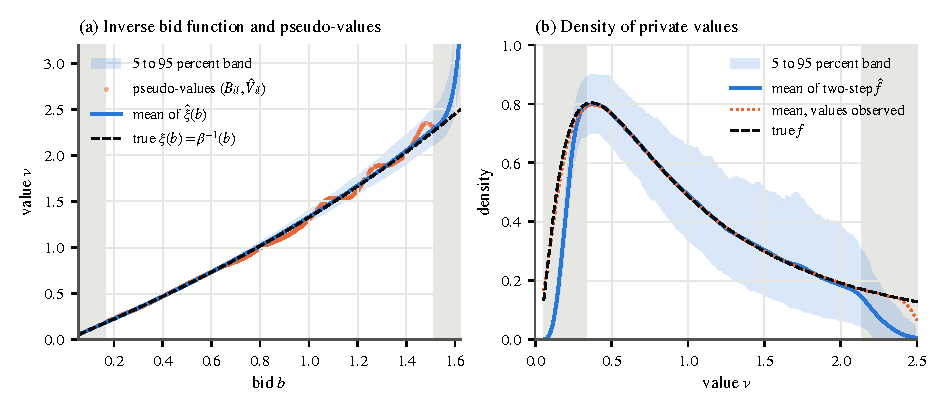
\includegraphics[width=\textwidth]{figures/appA/gpv.pdf}
\caption{The two-step estimator of \citet{GuerrePerrigneVuong2000} in their Monte Carlo design: 200
auctions with 5 bidders, values log-normal$(0,1)$ truncated to $[0.055,2.5]$, triweight kernels,
rule-of-thumb bandwidths, 1,000 replications. (a) True inverse bid function, mean and pointwise
5 to 95 percent band of $\hat\xi(b)$, and the pseudo-values of the first replication. The shaded bids are
trimmed on average (within $h_g$ of the extreme bids). (b) True value density, mean and pointwise
5 to 95 percent band of the two-step estimate, and the mean of the infeasible estimate from true values.
The shaded regions lie outside GPV's interior region (their footnote~9). Seed 20261022, script
\texttt{gpv\_mc.py}. Design follows Guerre, Perrigne and Vuong (2000), Section 2.4.}
\label{fig:A-gpv}
\end{figure}

The comparison with the infeasible estimator quantifies the price of inversion. On the interior region
the mean integrated squared error of the two-step estimate is 0.0170, against 0.0035 when values are
observed, a ratio of 4.9. The band in panel (b) is correspondingly wide, especially to the right of the
mode, where the bid density is low and its estimation error is amplified by \eqref{eq:A-gpv-xi}. Near
the lower end the two-step estimate collapses toward zero. Its mean at $v=0.055$ is 0.0003, against a
true density of 0.132. This is the joint effect of trimming and boundary bias, and it is why GPV report
results only on the interior region.

\section{Nonparametric regression, deconvolution and bounds}\label{sec:A-npreg}

This section estimates conditional means without functional form, combines nonparametric and
parametric components, separates a common factor from idiosyncratic noise, and draws inferences when
the data identify only a set. The tools build on \cref{sec:A-kde}. Throughout, $(y_i,x_i)$ are i.i.d.,
$m(x)=\E[y_i\mid x_i=x]$ is the regression function, $\sigma^2(x)=\Var(y_i\mid x_i=x)$, and $f$ is the
density of the scalar regressor $x_i$ unless stated otherwise.

\subsection{The Nadaraya-Watson estimator}\label{sec:A-nw}

The regression function is $m(x)=\frac{\int yf(x,y)\,\dd y}{f(x)}$. Replacing the joint density by the
product kernel estimate $\hat f(x,y)=\frac{1}{n}\sum_i\mathcal{K}_h(x-x_i)\mathcal{K}_h(y-y_i)$ and using
$\int y\,\mathcal{K}_h(y-y_i)\,\dd y=y_i$ for a symmetric kernel gives the \emph{Nadaraya-Watson
estimator} \citep{Nadaraya1964,Watson1964}:
\begin{equation}\label{eq:A-nw}
\hat m_h(x)=\frac{\sum_{i=1}^{n}\mathcal{K}_h(x-x_i)\,y_i}{\sum_{i=1}^{n}\mathcal{K}_h(x-x_i)} .
\end{equation}
It is a weighted average of the outcomes, with weights that decline with distance from $x$. It also
solves $\min_a\sum_i\mathcal{K}_h(x-x_i)(y_i-a)^2$, so it is a \emph{local constant} least squares fit.

\begin{proposition}[Bias and variance of Nadaraya-Watson]\label{prop:A-nw}
Let $x$ be an interior point with $f(x)>0$. Let $f$ be continuously differentiable and $m$ twice
continuously differentiable near $x$, let $\sigma^2$ be continuous, and let $h\to0$ and $nh\to\infty$.
Then
\begin{equation}\label{eq:A-nw-bias-var}
\E[\hat m_h(x)]-m(x)\approx h^2\mu_2\left(\frac{m''(x)}{2}+\frac{m'(x)f'(x)}{f(x)}\right),\qquad
\Var(\hat m_h(x))\approx\frac{\sigma^2(x)\kappa_2}{nhf(x)},
\end{equation}
where $\approx$ means equality of the leading terms.
\end{proposition}

\begin{proof}[Derivation]
Write $\hat m_h(x)-m(x)=\frac{\hat A(x)}{\hat f(x)}$ with
$\hat A(x)=\frac{1}{n}\sum_i\mathcal{K}_h(x-x_i)(y_i-m(x))$ and $\hat f(x)=\frac{1}{n}\sum_i\mathcal{K}_h(x-x_i)$.
Since $\hat f(x)\xrightarrow{p}f(x)$, the leading terms of the bias and variance are those of
$\frac{\hat A(x)}{f(x)}$.

\emph{Bias.} Using $\E[y_i\mid x_i]=m(x_i)$ and substituting $x_i=x-hu$,
\begin{equation*}
\E[\hat A(x)]=\int\mathcal{K}(u)\,\{m(x-hu)-m(x)\}\,f(x-hu)\,\dd u .
\end{equation*}
Expand $m(x-hu)-m(x)=-hum'(x)+\frac{h^2u^2}{2}m''(x)+o(h^2)$ and $f(x-hu)=f(x)-huf'(x)+o(h)$. The product
is $-hum'f+h^2u^2(m'f'+\frac{1}{2}m''f)+o(h^2)$. The term linear in $u$ integrates to zero, so
$\E[\hat A(x)]=h^2\mu_2(m'(x)f'(x)+\frac{1}{2}m''(x)f(x))+o(h^2)$. Dividing by $f(x)$ gives the bias.

\emph{Variance.} The leading term is
$\frac{1}{n}\E[\mathcal{K}_h(x-x_i)^2(y_i-m(x))^2]=\frac{1}{nh}\int\mathcal{K}(u)^2\{\sigma^2(x-hu)+(m(x-hu)-m(x))^2\}f(x-hu)\,\dd u$,
which equals $\frac{\kappa_2\sigma^2(x)f(x)}{nh}$ to first order. Dividing by $f(x)^2$ gives the variance.
\end{proof}

The bias has two parts. The curvature term $\frac{1}{2}m''$ is shared with every local smoother. The
\emph{design bias} $\frac{m'f'}{f}$ arises because, where the regressor density slopes, more
observations sit on one side of $x$ than on the other. The local average then leans toward the side
with more data, and the slope of $m$ converts the imbalance into bias.

At a boundary the problem is worse. Let the design have support $[0,\infty)$ with $f(0)>0$ and
evaluate at $x=0$. Only $u\le0$ contributes, so
$\E[\hat A(0)]\approx-hm'(0)f(0)\int_{-\infty}^{0}u\mathcal{K}(u)\,\dd u=hm'(0)f(0)\int_0^\infty u\mathcal{K}(u)\,\dd u$,
while $\hat f(0)\to\frac{1}{2}f(0)$. The bias is
\begin{equation}\label{eq:A-nw-boundary}
\E[\hat m_h(0)]-m(0)\approx2h\,m'(0)\int_0^\infty u\mathcal{K}(u)\,\dd u=\frac{3}{8}\,h\,m'(0)
\quad\text{(Epanechnikov kernel)},
\end{equation}
which is of order $h$ against $h^2$ in the interior. The Epanechnikov value
$\int_0^\infty u\mathcal{K}(u)\,\dd u=\frac{3}{16}$ is taken from \cref{tab:A-kernels}. For the four compact kernels of
that table the integral runs over $[0,1]$.

\subsection{Local polynomial regression}\label{sec:A-loclin}

The local constant fit ignores the slope of $m$. Fitting a line locally removes the design bias and the
first-order boundary bias. The \emph{local linear estimator} solves
\begin{equation}\label{eq:A-loclin}
(\hat a,\hat b)=\argmin_{a,b}\sum_{i=1}^{n}\mathcal{K}_h(x_i-x)\,\{y_i-a-b(x_i-x)\}^2,\qquad
\hat m_{\mathrm{LL}}(x)=\hat a .
\end{equation}
Let $S_j=\sum_i\mathcal{K}_h(x_i-x)(x_i-x)^j$. Solving the two normal equations gives
\begin{equation}\label{eq:A-loclin-weights}
\hat m_{\mathrm{LL}}(x)=\frac{\sum_iw_iy_i}{\sum_iw_i},\qquad w_i=\mathcal{K}_h(x_i-x)\{S_2-(x_i-x)S_1\}.
\end{equation}
The weights satisfy $\sum_iw_i(x_i-x)=S_1S_2-S_2S_1=0$. The estimator therefore reproduces any linear
function exactly, whatever the design.

\begin{proposition}[Local linear regression]\label{prop:A-loclin}
Let $\mathcal{K}$ vanish outside $[-1,1]$ and let $m$ be twice continuously differentiable. Conditional
on the regressors, and whenever $\sum_iw_i\ne0$,
\begin{equation*}
\E[\hat m_{\mathrm{LL}}(x)\mid x_1,\dots,x_n]-m(x)=\frac{\sum_iw_i\,\frac{1}{2}m''(\tilde x_i)(x_i-x)^2}{\sum_iw_i},
\end{equation*}
with $\tilde x_i$ between $x$ and $x_i$. Under the conditions of \cref{prop:A-nw}, the conditional bias at an
interior point is $\frac{h^2}{2}\mu_2m''(x)+o_p(h^2)$, free of the design term. At boundary points it remains of order
$h^2$. The interior variance is the Nadaraya-Watson variance $\frac{\sigma^2(x)\kappa_2}{nhf(x)}$
\citep{FanGijbels1996}.
\end{proposition}

\begin{proof}[Derivation]
Write $y_i=m(x)+m'(x)(x_i-x)+r_i+e_i$, where $r_i=\frac{1}{2}m''(\tilde x_i)(x_i-x)^2$ and
$\E[e_i\mid x_i]=0$. Substituting into \eqref{eq:A-loclin-weights}, the constant returns $m(x)$ and the
linear term vanishes because $\sum_iw_i(x_i-x)=0$. What remains is
$\frac{\sum_iw_i(r_i+e_i)}{\sum_iw_i}$, whose conditional mean is the displayed bias. Only observations
with $|x_i-x|\le h$ receive weight, so $|r_i|\le\frac{1}{2}h^2\sup|m''|$ wherever $x$ lies, and the bias
is $O_p(h^2)$ as long as $\frac{\sum_i|w_i|}{|\sum_iw_i|}$ stays bounded. That ratio is bounded at the
boundary too, because $S_0S_2-S_1^2>0$ when the window contains data on a set of positive length. In the
interior, $\frac{S_0}{n}\xrightarrow{p}f(x)$, $\E[\frac{S_1}{n}]=h^2\mu_2f'(x)+o(h^2)$ and $\Var(\frac{S_1}{n})=O(\frac{h}{n})$.
Hence $\frac{S_1}{S_0}=O_p(h^2+\sqrt{\frac{h}{n}})=o_p(h)$, because $\sqrt{\frac{h}{n}}=\frac{h}{\sqrt{nh}}$ and
$nh\to\infty$. The same calculation gives $\frac{S_2}{S_0}=h^2\mu_2+o_p(h^2)$. For $|x_i-x|\le h$ the
correction $\frac{(x_i-x)S_1}{S_2}$ in the weights is then $o_p(1)$. The weights therefore behave like
$\mathcal{K}_h(x_i-x)$ to first order, and the bias becomes $\frac{h^2}{2}\mu_2m''(x)$. The variance
argument is that of \cref{prop:A-nw}.
\end{proof}

Fitting a polynomial of degree $p$ in place of a line gives the \emph{local polynomial} estimator. The
coefficient on $(x_i-x)^k$ estimates $\frac{m^{(k)}(x)}{k!}$, so the slope $\hat b$ in
\eqref{eq:A-loclin} is a natural estimator of $m'(x)$. Odd degrees are preferred because they adapt
automatically to the boundary \citep{FanGijbels1996}.

\Cref{fig:A-npreg} compares the two estimators with the same Epanechnikov kernel and bandwidth $h=0.10$.
The design density is $\frac{2}{3}(1+x)$ on $[0,1]$ and the regression function is $m(x)=2e^{-5x}+0.5x$,
which is steep at the left boundary, with $m'(0)=-9.5$. With $n=400$, noise standard deviation 0.25 and
1,000 samples, the bias of Nadaraya-Watson at $x=0$ is $-0.316$. The approximation
\eqref{eq:A-nw-boundary} gives $-0.356$, and the difference reflects the large curvature of $m$ near
zero. The local linear bias at $x=0$ is $-0.028$. Its standard deviation there is larger, 0.105 against
0.064, because a line fitted at the edge extrapolates. In the interior both estimators share the
curvature bias, which reaches 0.031 for local linear near $x=0.1$, where $m''=50e^{-0.5}\approx30$.
Local fitting removes the design term and leaves the curvature term.

\begin{figure}[htbp]
\centering
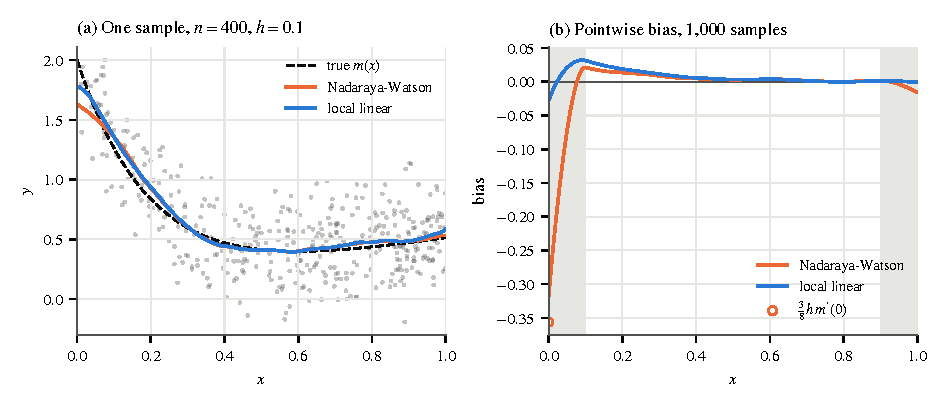
\includegraphics[width=\textwidth]{figures/appA/npreg.pdf}
\caption{Nadaraya-Watson and local linear regression with the same Epanechnikov kernel and bandwidth
$h=0.10$. The regressor has density $\frac{2}{3}(1+x)$ on $[0,1]$, $m(x)=2e^{-5x}+0.5x$, and the noise is
$N(0,0.25^2)$, $n=400$. (a) One sample. (b) Pointwise bias over 1,000 samples. The shaded
strips are within one bandwidth of the boundary, and the marker shows the boundary approximation
$\frac{3}{8}hm'(0)$ of \eqref{eq:A-nw-boundary}. Seed 20261022, script \texttt{npreg\_demo.py}.}
\label{fig:A-npreg}
\end{figure}

\casehead{Applications in the book}
Three applications use local regression. First, \citet{HausmanNewey1995} estimate demand $q(p,y)$
nonparametrically, as a function of price and income, and carry out the exact welfare analysis with it
\citep[fn.~6]{Hausman1997}. The exact analysis solves the differential equation of \citet{Hausman1981}. For a price change from
$p^0$ to $p^1$, let $S(p)=e(p,u^0)-y$ be the extra income needed to keep utility at its initial level.
Shephard's lemma and duality give
\begin{equation}\label{eq:A-hausman-ode}
\frac{\dd S(p)}{\dd p}=q\bigl(p,\,y+S(p)\bigr),\qquad S(p^0)=0,
\end{equation}
and the compensating variation is $S(p^1)$ (\cref{app:math}). \citet{Hausman1997} solves the same
differential equation for a parametric demand system for a new breakfast cereal. His exact welfare estimates and
their standard errors use the method of \citet{HausmanNewey1995} (his fn.~24, \cref{ch:newgoods}). Second, \citet[eq.~(18)]{BajariBenkard2005} recover
each product's unobserved characteristic as a conditional quantile. Normalizing $\xi$ to be uniform on
$[0,1]$ and independent of $x$, with price increasing in $\xi$, they set
$\hat\xi_{jt}=\hat F_{p_t\mid x=x_j}(p_{jt})$. In their application a local linear kernel estimator
\citep{FanGijbels1996} with a normal kernel worked best \citep[Sections~5.1 and~6]{BajariBenkard2005}.
Derivatives of the estimated hedonic price function then recover consumers' marginal valuations from
their first-order conditions (\cref{ch:discrete}). Third, conditional bid distributions given covariates
can be estimated by local linear smoothing of indicator outcomes $\indic\{B_{il}\le b\}$, which avoids
the boundary problems of \cref{sec:A-kde-boundary} in the covariate dimension.

\subsection{Series and sieve estimators}\label{sec:A-series}

A \emph{series estimator} approximates $m$ by a linear combination of $K_n$ known basis functions
$\psi(x)=(\psi_1(x),\dots,\psi_{K_n}(x))^\top$, such as powers of $x$ or regression splines. A regression
spline of degree $r$ is a polynomial of degree $r$ between consecutive points called knots, with $r-1$ continuous
derivatives at each knot. B-splines are a convenient basis for this space. The series estimator fits the
coefficients by least squares,
\begin{equation}\label{eq:A-series}
\hat m(x)=\psi(x)^\top\hat\gamma,\qquad \hat\gamma=(\Psi^\top\Psi)^{-1}\Psi^\top y .
\end{equation}
Here $\Psi$ is the $n\times K_n$ matrix with rows $\psi(x_i)^\top$. The number of terms plays the role of
the inverse bandwidth. Its variance cost has an exact expression. With homoskedastic errors of variance
$\sigma^2$, the fitted values are $P_\Psi y$ with $P_\Psi=\Psi(\Psi^\top\Psi)^{-1}\Psi^\top$, so
\begin{equation*}
\frac{1}{n}\sum_{i=1}^{n}\Var(\hat m(x_i)\mid\Psi)=\frac{\sigma^2}{n}\,\mathrm{tr}(P_\Psi)=\frac{\sigma^2K_n}{n}.
\end{equation*}
For a function with $R$ derivatives and a polynomial or spline basis in one dimension, the squared
approximation bias is of order $K_n^{-2R}$. Balancing the two gives $K_n\propto n^{\frac{1}{2R+1}}$ and the
same mean squared error rate $n^{-\frac{2R}{2R+1}}$ as a kernel estimator \citep{Newey1997}. In practice
$K_n$ is chosen by cross-validation or an information criterion.

Series estimators are global. A misbehaving term affects the fit everywhere, and high-order
polynomials are unstable at the boundary, which favors splines. In exchange, restrictions such as
additivity, $m(x)=m_1(x_1)+m_2(x_2)$, are easy to impose by choosing the basis, and the estimator is a
least squares regression whose inference is standard for fixed $K_n$. A \emph{sieve} is the general
version. It is a sequence of increasingly rich approximating function classes, and the estimator uses a richer
class as $n$ grows \citep{Chen2007}. Three uses appear in
the book. Approximations to optimal instruments use series in the instruments (\cref{sec:A-optimal-iv}).
The marginal cost of an airline segment in \citet{BerryCarnallSpiller1996} is a cubic polynomial in leg
distance and leg density, with two congestion shifters (WP Table~5, \cref{sec:09-bcs-supply}). It is a
fixed low-order series. And
\citet[footnote~20]{AtheyHaile2007} point to sieve estimation as a practical alternative to kernels
in auctions with observed heterogeneity.

\subsection{The partially linear model}\label{sec:A-plm}

Often only a few parameters are of interest, while a control variable enters in an unknown way. The
\emph{partially linear model} is
\begin{equation}\label{eq:A-plm}
y_i=x_i^\top\beta+m(w_i)+e_i,\qquad \E[e_i\mid x_i,w_i]=0,
\end{equation}
with $m$ unknown. Taking expectations conditional on $w_i$ gives
$\E[y_i\mid w_i]=\E[x_i\mid w_i]^\top\beta+m(w_i)$. Subtracting this from \eqref{eq:A-plm} eliminates
$m$:
\begin{equation}\label{eq:A-robinson}
\tilde y_i=\tilde x_i^\top\beta+e_i,\qquad \tilde y_i=y_i-\E[y_i\mid w_i],\quad \tilde x_i=x_i-\E[x_i\mid w_i].
\end{equation}
\citet{Robinson1988} estimates the two conditional means nonparametrically and regresses the
residual of $y$ on the residual of $x$ by least squares. This is the \emph{double-residual estimator}.

\begin{proposition}[Robinson's estimator]\label{prop:A-robinson}
Suppose $\E[\tilde x_i\tilde x_i^\top]$ is positive definite, so no linear combination of $x_i$ is a
function of $w_i$ alone. Suppose the first-step estimators of $\E[y\mid w]$ and $\E[x\mid w]$ converge
in mean square faster than $n^{-\frac{1}{4}}$, with trimming and kernel order as in
\citet{Robinson1988}. Then
\begin{equation*}
\sqrt n(\hat\beta-\beta)\xrightarrow{d}N\!\left(0,\ \E[\tilde x\tilde x^\top]^{-1}\E[e^2\tilde x\tilde x^\top]\E[\tilde x\tilde x^\top]^{-1}\right),
\end{equation*}
the distribution of the infeasible regression with known conditional means.
\end{proposition}

\begin{proof}[Why the first step does not matter]
The estimator solves the sample analogue of the moment
$\E[(\tilde y-\tilde x^\top\beta)\tilde x]=0$. Perturb the conditional means by functions $\delta_y(w)$
and $\delta_x(w)$, so the moment becomes
$M(\delta)=\E[\{\tilde y-\delta_y(w)-(\tilde x-\delta_x(w))^\top\beta\}\{\tilde x-\delta_x(w)\}]$. Its
derivative at $\delta=0$ in the direction $\delta_y$ is $-\E[\delta_y(w)\tilde x]$, which is zero because
$\E[\tilde x\mid w]=0$. In the direction $\delta_x$ the derivative is
$\E[\tilde x\,\delta_x(w)^\top]\beta-\E[e\,\delta_x(w)]$, and both terms vanish by
$\E[\tilde x\mid w]=0$ and $\E[e\mid w]=0$. First-step errors therefore enter only through products of
two errors, of order $\|\hat\delta\|^2$. If $\|\hat\delta\|=o_p(n^{-\frac{1}{4}})$, these products are
$o_p(n^{-\frac{1}{2}})$, and the infeasible limit applies.
\end{proof}

The estimator is the nonparametric analogue of the Frisch-Waugh-Lovell theorem (\cref{thm:A-fwl}). If
$m(w)=w^\top\gamma$, partialling out $w$ by linear projection and regressing residual on residual
reproduces the coefficient on $x$ in the long regression. Robinson replaces the linear projection by
the conditional expectation, which partials out every function of $w$. The insensitivity to the first
step derived in the proof is the property now called \emph{Neyman orthogonality}.

A simulation in \texttt{npreg\_demo.py} shows what is at stake. Let $w$ be uniform on $[0,1]$,
$x=\sin(2\pi w)+v$ and $y=x+2\sin(2\pi w)+e$, with $v$ and $e$ standard normal, $n=500$ and 1,000 samples.
Least squares of $y$ on a constant, $x$ and $w$ controls for $w$ linearly. Its mean estimate is 1.327
against $\beta=1$, and its nominal 95 percent interval never covers the truth. Robinson's estimator with
local linear first steps ($h=0.08$) has mean 0.999 and standard deviation 0.045, equal to the infeasible
value $\frac{1}{\sqrt{500}}\approx0.045$. Its interval covers in 94.1 percent of samples.

\subsection{Deconvolution}\label{sec:A-deconv}

Suppose two noisy measurements share a common component,
\begin{equation}\label{eq:A-meas}
Y_1=U+\epsilon_1,\qquad Y_2=U+\epsilon_2,
\end{equation}
with $U$, $\epsilon_1$ and $\epsilon_2$ mutually independent. In auctions, $U$ is the log of a factor that
scales all bids in an auction, known to the bidders and unobserved by us. The term $\epsilon_j$ is the log of the
bid that bidder $j$ would make if the factor were one. The goal is the distribution of each
component from the joint distribution of $(Y_1,Y_2)$.

Second moments show why two measurements help. Independence gives $\Cov(Y_1,Y_2)=\Var(U)$, so
$\Var(\epsilon_j)=\Var(Y_j)-\Cov(Y_1,Y_2)$, and the normalization $\E[\epsilon_1]=0$ gives
$\E[U]=\E[Y_1]$. Variation across auctions identifies the spread of the common factor, and variation
within auctions identifies the spread of the idiosyncratic parts. A theorem of \citet{Kotlarski1966}
extends this from second moments to whole distributions. Let
$\varphi_U(t)=\E[e^{\mathrm{i}tU}]$ denote a characteristic function, where $\mathrm{i}$ is the
imaginary unit, and let $\varphi_{Y_1Y_2}(t_1,t_2)=\E[e^{\mathrm{i}t_1Y_1+\mathrm{i}t_2Y_2}]$.

\begin{lemma}[Kotlarski]\label{lem:A-kotlarski}
In \eqref{eq:A-meas}, let $U$, $\epsilon_1$, $\epsilon_2$ be mutually independent with finite first
moments and $\E[\epsilon_1]=0$, and let $\varphi_U$ and $\varphi_{\epsilon_2}$ never vanish. Then for every
real $t$,
\begin{equation}\label{eq:A-kotlarski}
\varphi_U(t)=\exp\left(\int_0^t\frac{\E\left[\mathrm{i}Y_1e^{\mathrm{i}sY_2}\right]}{\E\left[e^{\mathrm{i}sY_2}\right]}\,\dd s\right),\qquad
\varphi_{\epsilon_1}(t)=\frac{\varphi_{Y_1Y_2}(t,0)}{\varphi_U(t)},\qquad
\varphi_{\epsilon_2}(t)=\frac{\varphi_{Y_1Y_2}(0,t)}{\varphi_U(t)} .
\end{equation}
The joint distribution of $(Y_1,Y_2)$ therefore determines the distributions of $U$, $\epsilon_1$ and
$\epsilon_2$.
\end{lemma}

\begin{proof}
Independence factors the joint characteristic function:
\begin{equation*}
\varphi_{Y_1Y_2}(t_1,t_2)=\E\left[e^{\mathrm{i}(t_1+t_2)U}e^{\mathrm{i}t_1\epsilon_1}e^{\mathrm{i}t_2\epsilon_2}\right]
=\varphi_U(t_1+t_2)\,\varphi_{\epsilon_1}(t_1)\,\varphi_{\epsilon_2}(t_2).
\end{equation*}
Finite first moments make the characteristic functions continuously differentiable, with
$\varphi_X'(0)=\mathrm{i}\E[X]$. Differentiating in $t_1$ and setting $t_1=0$, with $\varphi_{\epsilon_1}(0)=1$
and $\varphi_{\epsilon_1}'(0)=\mathrm{i}\E[\epsilon_1]=0$,
\begin{equation*}
\frac{\partial\varphi_{Y_1Y_2}}{\partial t_1}(0,s)=\varphi_U'(s)\,\varphi_{\epsilon_2}(s).
\end{equation*}
The left side equals $\E[\mathrm{i}Y_1e^{\mathrm{i}sY_2}]$, and $\varphi_{Y_1Y_2}(0,s)=\E[e^{\mathrm{i}sY_2}]=\varphi_U(s)\varphi_{\epsilon_2}(s)\ne0$.
Dividing, $\varphi_{\epsilon_2}(s)$ cancels:
\begin{equation*}
\frac{\E[\mathrm{i}Y_1e^{\mathrm{i}sY_2}]}{\E[e^{\mathrm{i}sY_2}]}=\frac{\varphi_U'(s)}{\varphi_U(s)}=\frac{\dd}{\dd s}\log\varphi_U(s),
\end{equation*}
where $\log$ is the continuous branch with $\log\varphi_U(0)=0$, which exists because $\varphi_U$ is
continuous and never zero. Integrating from 0 to $t$ and exponentiating gives the first formula. Setting
$t_2=0$, and then $t_1=0$, in the factorization gives $\varphi_{Y_1Y_2}(t,0)=\varphi_U(t)\varphi_{\epsilon_1}(t)$ and
$\varphi_{Y_1Y_2}(0,t)=\varphi_U(t)\varphi_{\epsilon_2}(t)$, and division gives the other two. A characteristic
function determines its distribution.
\end{proof}

Each assumption has a role. Independence delivers the factorization. The nonvanishing condition allows
the divisions and the logarithm. The zero mean of $\epsilon_1$ is a location normalization, since a
constant could otherwise move freely between $U$ and the $\epsilon$'s. The lemma identifies
distributions only. The realization of $U$ in a given auction is not identified. \Cref{ch:collusion-evidence} states
the same result for Asker's application.

The nonvanishing condition deserves care. \citet[Lemma~1]{Krasnokutskaya2011} argues that a variable
with bounded support has a characteristic function that extends to an entire function, so its zeros are
isolated. Isolated zeros can still occur, as the uniform distribution shows, since its characteristic
function $\frac{\sin t}{t}$ vanishes at multiples of $\pi$. \citet{EvdokimovWhite2012} show that
identification survives some violations of the condition under additional restrictions.

\casehead{The estimator}
\citet{LiVuong1998} replace each characteristic function by its sample analogue. With $n$ independent
pairs $(Y_{1k},Y_{2k})$,
\begin{equation}\label{eq:A-lv}
\hat\varphi_U(t)=\exp\left(\int_0^t\frac{\frac{1}{n}\sum_k\mathrm{i}Y_{1k}e^{\mathrm{i}sY_{2k}}}{\frac{1}{n}\sum_ke^{\mathrm{i}sY_{2k}}}\,\dd s\right),\qquad
\hat f_U(u)=\frac{1}{2\pi}\int_{-T}^{T}d_T(t)\,e^{-\mathrm{i}tu}\,\hat\varphi_U(t)\,\dd t ,
\end{equation}
and analogously for $\epsilon_1$ and $\epsilon_2$. The density is recovered by the inverse Fourier
transform, truncated at $\pm T$ and multiplied by a \emph{damping factor} $d_T$ that downweights high
frequencies, such as $d_T(t)=\max\{1-\frac{|t|}{T},0\}$ \citep{DiggleHall1993}. Since
$\hat\varphi_U(-t)$ is the complex conjugate of $\hat\varphi_U(t)$, the estimate is real and equals
$\frac{1}{\pi}\int_0^Td_T(t)\,\mathrm{Re}\{e^{-\mathrm{i}tu}\hat\varphi_U(t)\}\,\dd t$. The truncation
point $T$ is the smoothing parameter, playing the role of an inverse bandwidth.

Deconvolution converges slowly. The empirical characteristic function has error of order
$n^{-\frac{1}{2}}$ at each frequency, but the formulas divide by quantities that decay at high
frequencies. The ratio in \eqref{eq:A-lv} divides by $\varphi_U(s)\varphi_{\epsilon_2}(s)$, and the formula
for $\varphi_{\epsilon_1}$ divides by $\varphi_U$. The achievable rate depends on how fast the characteristic
functions decay. It is polynomial in $n$ for \emph{ordinary smooth} distributions, whose characteristic
functions decay like $|t|^{-\beta}$, and only logarithmic for \emph{supersmooth} ones such as the normal
\citep{Fan1991}. \citet{LiVuong1998} establish uniform consistency under conditions of this kind.
Krasnokutskaya's consistency result assumes ordinary smooth components with $\beta>1$
\citep[Proposition~5]{Krasnokutskaya2011}.

\Cref{fig:A-deconv} implements \eqref{eq:A-lv} with $U$ distributed Gamma with shape 4 and scale 0.25
(mean 1, standard deviation 0.5), $\epsilon_j\sim N(0,0.4^2)$, $n=1{,}000$ pairs and 200 samples. With
$T=8$ the median integrated squared error of $\hat f_U$ is 0.035. A kernel density estimate of $Y_1$
ignores the noise and has mean integrated squared error 0.058. Raising $T$ to 10 lowers the median
error to 0.029 but makes the estimator unstable, with a mean integrated squared error of 2.44 driven by
a few samples. Too large a $T$ divides by empirical characteristic functions that are pure noise.

\begin{figure}[htbp]
\centering
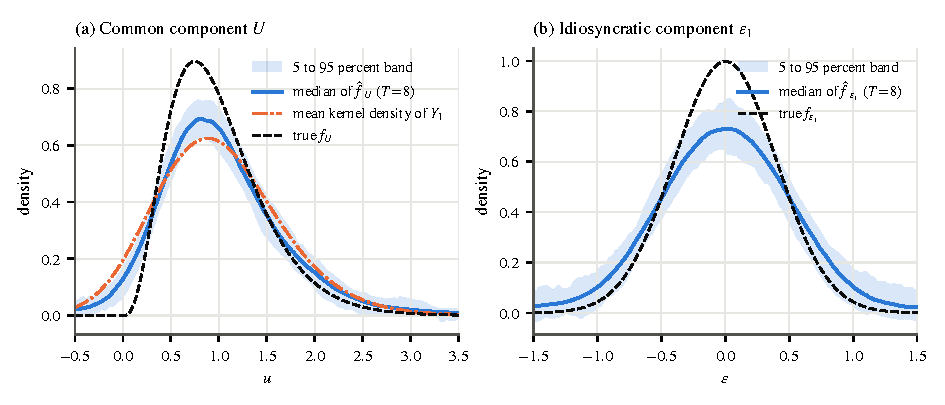
\includegraphics[width=\textwidth]{figures/appA/deconv.pdf}
\caption{Kotlarski deconvolution with the estimator of \citet{LiVuong1998}. $Y_j=U+\epsilon_j$ with
$U\sim\mathrm{Gamma}(4,0.25)$ and $\epsilon_j\sim N(0,0.4^2)$, $n=1{,}000$ pairs, smoothing parameter
$T=8$, damping factor $1-\frac{|t|}{T}$, 200 samples. (a) True density of $U$, pointwise median
and 5 to 95 percent band of $\hat f_U$, and the mean rule-of-thumb kernel density estimate of $Y_1$.
(b) The same for $\epsilon_1$. Seed 20261022, script \texttt{npreg\_demo.py}.}
\label{fig:A-deconv}
\end{figure}

\casehead{Krasnokutskaya's procurement auctions}
\citet{Krasnokutskaya2011} applies the lemma to first-price procurement auctions. A bidder's cost is
the product of a project-level component $Y$, common knowledge among bidders and unobserved by us, and an
individual component. The equilibrium bid inherits the product structure, $B_{ij}=y_ja_{ij}$, where
$a_{ij}$ is the bid at $y=1$. For two bidders in the same auction, logs give
$\log B_{i_1}=\log Y+\log A_{i_1}$ and $\log B_{i_2}=\log Y+\log A_{i_2}$. Her equation~(3) is
\eqref{eq:A-kotlarski} for these variables.\footnote{Its equation~(3) prints a logarithm where the
exponential of \eqref{eq:A-kotlarski} belongs. The estimator in its appendix uses the exponential.} The
location is fixed by $\E[\log A_1]=0$. Her estimator averages the empirical characteristic function over
all pairs of bidders of the relevant types. It scales bids into $[0,2]$ to reduce estimation error in the
characteristic function. It uses the damping factor $1-\frac{|t|}{T}$ and chooses $T$ to match the means
and variances of $\log Y$ and $\log A$ implied by the bids, which selects $T=50$ in her application. The
moment conditions behind the choice of $T$ are the second-moment identities above. With identically
distributed individual components, $\Var(\log A)=\frac{1}{2}\E[(\log B_1-\log B_2)^2]$ and
$\Var(\log Y)=\Var(\log B)-\Var(\log A)$ \citep[Section~4.3]{Krasnokutskaya2011}. In a second step she
draws pseudo-bids from the estimated density of the individual component by rejection sampling. She
converts them to pseudo-costs through the asymmetric first-order condition. The densities in this step
use a triweight kernel and the bandwidth $2.978\times1.06\,\hat\sigma L^{-\frac{1}{6}}$, where
$\hat\sigma$ is the standard deviation of the log of one plus the bids. Confidence intervals come from
the bootstrap. Independence also generates testable restrictions. The characteristic functions
recovered from different pairs and triples of bidders must agree. A degenerate $\log Y$ gives the
independent private values model, which can be tested within the same framework (her conditions W1 to
W7). In Michigan highway procurement auctions she attributes about 75 percent of the variation in
bidders' costs to factors known to all bidders. Only 25 percent comes from private information
(abstract of the working paper). \citet[p.~103]{HortacsuPerrigne2021} report the published estimate as 34 percent
of the bid variation from private information. That figure refers to bids, while the working-paper figure refers to
costs. \Cref{ch:auction-empirics} discusses the application.

\casehead{Asker's knockout bids}
\citet{Asker2010} applies the same estimator to pairs of normalized knockout bids in a stamp-dealer ring,
$\ln\hat b_{1k}=\ln(\varepsilon_k)+\ln\beta(v_{1k})$ and $\ln\hat b_{2k}=\ln(\varepsilon_k)+\ln\beta(v_{2k})$
(his eq.~(4)). In his notation the common component of lot $k$ is $\ln(\varepsilon_k)$, which plays the
role of $U$ in \eqref{eq:A-meas}. He imposes $\E[\ln\beta(v_1)]=0$ and independence (his Assumption~U).
The target-auction price supplies a third measurement of the common component. He averages the estimated characteristic
functions from the two kinds of pairs, weighting by the number of observations of each, as
\citet{LiVuong1998} suggest. His damping factor is $\max\{1-\frac{|t|}{\sqrt2T_n},0\}$. The smoothing
parameter is $T_n=50$ for the common component, whose estimate proved insensitive to it. For the strong
members, the weak members and the highest non-ring value, the values 12.0, 3.0 and 8.3 minimize a
criterion. The criterion matches naive damages and the ring's win probability and penalizes
non-monotone bid functions \citep[pp.~748--749]{Asker2010}. As with Krasnokutskaya, only distributions are identified, and
the GPV inversion is applied to draws from the estimated distributions (\cref{ch:collusion-evidence}).

\subsection{Estimation and inference under partial identification}\label{sec:A-partialid}

When the model and data restrict a parameter only to a set, the parameter is \emph{partially identified}
(\cref{def:A-identification}). A common form is a set of moment inequalities,
\begin{equation}\label{eq:A-mi}
\Theta_I=\{\theta\in\Theta:\ \E[m_j(W;\theta)]\ge0,\ j=1,\dots,J\},
\end{equation}
where $\Theta_I$ is the \emph{identified set}. Every point of $\Theta_I$ is consistent with the population
distribution of the data, and no point outside it is. Estimation targets the set, and inference can
target either the set or the true parameter inside it.

\casehead{Bounds in English auctions}
\citet{HaileTamer2003} drop the button-auction model of ascending auctions, in which bidders exit at
their values. They impose two behavioral assumptions. Bidders never bid more than their value, and
bidders never let an opponent win at a price they would have been willing to beat. Let $G_{k:n}$ be the
distribution of the $k$-th lowest bid in $n$-bidder auctions. Let $G^{\Delta}_{n:n}$ be the distribution
of the winning bid plus the minimum increment $\Delta$, and $\phi_{k:n}$ the map from $F$ to $F_{(k:n)}$
in \eqref{eq:A-orderstat}. The first assumption implies that the $k$-th lowest bid is at most the $k$-th
lowest value, so $G_{k:n}(v)\ge\phi_{k:n}(F(v))$. The second implies that the second-highest value is at
most the winning bid plus $\Delta$, so $\phi_{n-1:n}(F(v))\ge G^{\Delta}_{n:n}(v)$. Inverting the
increasing maps and combining all order statistics and all $n$ gives
\citep[Section~4.3.1, eqs.~(4.10)--(4.11)]{AtheyHaile2007}
\begin{equation}\label{eq:A-ht}
F^-(v)=\max_n\ \phi_{n-1:n}^{-1}\!\left(G^{\Delta}_{n:n}(v)\right)\ \le\ F(v)\ \le\
F^+(v)=\min_{n}\min_{1\le k\le n}\ \phi_{k:n}^{-1}\!\left(G_{k:n}(v)\right).
\end{equation}
\Cref{ch:auction-empirics} develops the bounds and their use for reserve prices.
\citet[pp.~493--499]{AradillasLopezGandhiQuint2013} derive bounds on expected profit, bidder surplus and
the optimal reserve price when symmetric private values have nonnegative dependence. They use only the transaction price and,
with values independent of the number of bidders, variation in that number across auctions.
\citet[footnote~37]{Asker2010}
discusses why he does not use the Haile-Tamer approach. Jump bidding was rare at the stamp auctions he
observed, and bid increments were small relative to bids.

\casehead{Plug-in estimation and the bias of extrema}
The natural estimator of \eqref{eq:A-ht} replaces each $G$ by an empirical distribution function. The
minimum and maximum then create a finite-sample bias. The minimum is concave, so by Jensen's inequality
$\E[\min_j\hat a_j]\le\min_j\E[\hat a_j]$. A worked case shows the size. Let $\hat a_1$ and $\hat a_2$ be
independent $N(a,\sigma^2)$, both unbiased for the same bound $a$. Since $\min(a_1,a_2)=\frac{a_1+a_2}{2}-\frac{|a_1-a_2|}{2}$
and $\hat a_1-\hat a_2\sim N(0,2\sigma^2)$ has mean absolute value $\frac{2\sigma}{\sqrt\pi}$,
\begin{equation*}
\E\left[\min(\hat a_1,\hat a_2)\right]=a-\frac{\sigma}{\sqrt\pi}.
\end{equation*}
The estimated upper bound is too low and the estimated lower bound too high, so the estimated set is too
narrow. The bias grows with the number of terms in the minimum. \citet{HaileTamer2003} define the
bounds in finite samples with smooth approximations to the max and min functions. In the words of
\citet[Section~4.3.1, p.~35]{AtheyHaile2007}, this ``amounts to using weighted averages instead of the max or min.''
For example, the softmax-weighted average
$\sum_j\hat a_j\frac{e^{\rho\hat a_j}}{\sum_ke^{\rho\hat a_k}}$ with $\rho<0$ is a smooth minimum of
this kind. It tends to $\min_j\hat a_j$ as $\rho\to-\infty$, and it lies above the minimum, which
offsets the downward bias. We use it only as an illustration, and it need not be the weighting that Haile
and Tamer choose.

The extrema also break standard inference. The functional $\min(a_1,a_2)$ is not differentiable where
$a_1=a_2$, so the delta method fails there, and the bootstrap can fail for the same reason
(\cref{prop:A-boot-max}).

\casehead{Set estimators and confidence regions}
Define the criterion $Q(\theta)=\sum_j(\min\{\E[m_j(W;\theta)],0\})^2$, which is zero exactly on
$\Theta_I$. Its sample analogue $Q_n$ is zero on the sample identified set, which may be empty or too
small. \citet{ChernozhukovHongTamer2007} estimate the set by $\hat\Theta_I=\{\theta:\ nQ_n(\theta)\le c_n\}$
with $c_n\to\infty$ and $\frac{c_n}{n}\to0$. The Hausdorff distance between sets $A$ and $B$ is
\begin{equation*}
d_H(A,B)=\max\Bigl\{\sup_{a\in A}\inf_{b\in B}\lVert a-b\rVert,\ \sup_{b\in B}\inf_{a\in A}\lVert a-b\rVert\Bigr\}.
\end{equation*}
It is the larger of two directed distances. Each is the largest distance from a point of one set to the nearest
point of the other. The estimator is consistent in this distance, so $d_H(\hat\Theta_I,\Theta_I)\to0$ in
probability. Confidence regions
for $\Theta_I$ invert tests of $Q(\theta)=0$, with cutoffs from subsampling or the bootstrap.

For an interval $[\theta_l,\theta_u]$ there is an important distinction. A region that covers the whole
set with probability $1-\alpha$ is larger than one that covers the true parameter with that probability.
\citet{ImbensManski2004} construct the second kind. With estimators $\hat\theta_l$ and $\hat\theta_u$,
standard errors $\frac{\hat\sigma_l}{\sqrt n}$ and $\frac{\hat\sigma_u}{\sqrt n}$, and estimated length
$\hat\Delta=\hat\theta_u-\hat\theta_l$, the interval is
\begin{equation}\label{eq:A-im}
\left[\hat\theta_l-c_n\frac{\hat\sigma_l}{\sqrt n},\ \hat\theta_u+c_n\frac{\hat\sigma_u}{\sqrt n}\right],\qquad
\Phi\!\left(c_n+\frac{\sqrt n\,\hat\Delta}{\max\{\hat\sigma_l,\hat\sigma_u\}}\right)-\Phi(-c_n)=1-\alpha .
\end{equation}
When the set is long relative to sampling error, the true parameter can be near at most one end point.
Only one tail then matters, and $c_n$ approaches the one-sided value 1.645 for $\alpha=0.05$. When the set
shrinks to a point, $c_n$ rises to the two-sided 1.96. A region for the whole set needs both end
points covered at once and uses a larger constant. \citet{Stoye2009} refines the argument for sets whose
length is near zero. \citet{Manski2003} and \citet{Tamer2010} survey the field.
